\documentclass[11pt,a4paper]{article}

\usepackage[T1]{fontenc}
\usepackage[utf8]{inputenc}
\usepackage{lmodern}
\usepackage{microtype}
\usepackage[margin=2.4cm]{geometry}
\usepackage{amsmath,amssymb,amsthm}
\usepackage{booktabs}
\usepackage{graphicx}
\usepackage{longtable}
\usepackage{siunitx}
\usepackage{xcolor}
\usepackage[hidelinks]{hyperref}
\usepackage{caption}
\usepackage{enumitem}
\usepackage{fancyhdr}
\usepackage{fancyvrb}

\captionsetup{font=small,labelfont=bf}
\emergencystretch=2.5em
\setlength{\parindent}{0pt}
\setlength{\parskip}{0.45em}
\setlist{nosep,leftmargin=1.4em}

\newtheorem{theorem}{Theorem}[section]
\newtheorem{corollary}[theorem]{Corollary}
\newtheorem{lemma}[theorem]{Lemma}
\newtheorem{remark}[theorem]{Remark}
\theoremstyle{definition}
\newtheorem{definition}[theorem]{Definition}

\newcommand{\Omm}{\Omega_{\mathrm{m}}}
\newcommand{\Omr}{\Omega_{\mathrm{r}}}
\newcommand{\OmL}{\Omega_{\Lambda}}
\newcommand{\Hzt}{H_0 t_0}
\newcommand{\gamm}{\gamma}
\newcommand{\muc}{\mu(k,a)}
\newcommand{\kms}{\,\mathrm{km\,s^{-1}\,Mpc^{-1}}}
\newcommand{\Mpc}{\,\mathrm{Mpc}}

\pagestyle{fancy}
\fancyhf{}
\fancyhead[L]{\small RATISS Verse I}
\fancyhead[R]{\small\thepage}
\renewcommand{\headrulewidth}{0.3pt}

\title{\vspace{-1.2cm}\textbf{RATISS Verse I}\\[0.3em]
\large A sealed, falsifiable reference atlas of ten cosmological universes}

\author{Jonathan Evina\thanks{\raggedright RATISS Labs, Yaound\'e, Cameroon. ORCID 0009-0000-4092-5313. Correspondence: \texttt{jonathan.ratisslabs@zohomail.com}.}}
\date{30 October 2026 \quad\textbullet\quad Version 1.0.0}

\begin{document}

\maketitle

\begin{abstract}
\noindent
We present \textsc{Ratiss Verse I}, a reference atlas in which ten distinct
cosmological models are integrated through a \emph{single} solver chain: one
background quadrature, one linear growth equation, and one particle--mesh
$N$-body engine. Every number in the atlas is recomputed from a frozen
parameter set at build time; nothing is transcribed by hand; every produced
artefact is sealed with a SHA-256 manifest.

The atlas is built to answer one question honestly: \emph{which of these ten
universes is actually distinguishable from $\Lambda$CDM?} Our answer is
uncomfortable. Six models --- $\Lambda$CDM, $f(R)$ Hu--Sawicki, $f(T)$
teleparallel, a running-vacuum model with $\nu=10^{-3}$, a constant-$w$ fluid
at $w=-1.004$, and the RATISS granular universe --- agree on $H_0t_0$ to
within $5.6\times10^{-4}$ ($0.06\%$). The dimensionless age is therefore
\emph{degenerate} and cannot serve as a discriminator. The growth index
$\gamm$ separates them at the $6.7\%$ level ($0.5542 \to 0.5916$), which is
within reach of stage-IV surveys.

We report four analytic results and one negative result of some weight. The
negative result concerns the widely quoted target $H_0t_0 = 0.9549$: we show
it is not a property of any equation of state but of \emph{emptiness}. A
universe containing a single substance with $\rho \propto a^{-n}$ has
$\Hzt = 2/n$ exactly; with $n = 2.0945$ this gives $0.95488$. Adding the
matter that galaxies require drives $\Hzt$ down to $0.7927$, an age of
$11.51$~Gyr, below the age of the oldest stars. Reproducing $0.9549$ with
matter present requires a \emph{phantom} equation of state, $w = -1.0332$,
or $\Omm = 0.3100$.

We also report the defects we found in our own pipeline, including a
radiation-inconsistency between model families that shifted $\Hzt$ by
$3.8\times10^{-4}$ --- larger than several effects the atlas was built to
resolve --- and we give the corrected values throughout.

Every figure, table and hash in this document can be regenerated with one
command. The repository is the artefact.
\end{abstract}

\vspace{0.5em}
\noindent\textbf{Keywords:} cosmology --- dark energy --- modified gravity ---
$N$-body simulation --- reproducibility --- falsifiability --- open science

\tableofcontents
\newpage

%======================================================================
\section{Introduction}
\label{sec:intro}

\subsection{The problem this atlas addresses}

Cosmological model building has an asymmetry problem. It is cheap to write
down a modification of general relativity that fits the expansion history;
it is expensive, and rarely done, to state in advance what measurement would
kill it. The literature contains a large number of models whose predictions
differ from $\Lambda$CDM at a level the models themselves do not quantify.

This atlas was built to make that quantification mechanical. Ten models are
declared. Each is reduced to three ingredients:

\begin{enumerate}[label=(\roman*)]
\item a background expansion rate $E(a) = H(a)/H_0$;
\item a linear growth history, driven by an effective coupling $\muc$;
\item a local force law, entering the $N$-body engine through the same
      $\muc$.
\end{enumerate}

Given those three, every observable quantity used here follows from two
solvers and one simulation. No model is allowed a bespoke derivation. This
is the central design decision: \emph{one code path, ten universes}.

\subsection{Lineage}

The atlas is the direct successor of a toy model, \textsc{Syntoron 24}, which
integrated $24$ particles under the pair force
\begin{equation}
F(r) = -\frac{G}{r^2} + \frac{K}{r^4},
\qquad r_c \equiv \sqrt{K/G},
\label{eq:force}
\end{equation}
and reported a single dimensionless number, $H t = 1$. The toy was internally
consistent and externally unfalsifiable: it had no expansion history, no
spectrum, and no observational contact.

\textsc{Ratiss Verse I} keeps the force law of Eq.~\eqref{eq:force} --- it is
the only content of the toy that survived --- and embeds it in a cosmological
setting where it has consequences (Section~\ref{sec:granular}). Everything
else in the toy is retired.

\subsection{What is new here}

\begin{itemize}
\item A \emph{registry} of ten universes sharing one solver chain, with every
      number regenerated at build time
      (\texttt{scripts/build.py}, 26.6~s wall clock).
\item Three analytic results (Section~\ref{sec:analytic}) that constrain what
      a cut-off can and cannot do.
\item A negative result of general interest: the $0.9549$ target that
      motivated a family of single-fluid models is an artefact of the absence
      of matter (Section~\ref{sec:negative}).
\item A documented list of the defects found in our own pipeline, with the
      corrected numbers
      (Section~\ref{sec:defects} and Appendix~\ref{app:defects}).
\item Cryptographic sealing: twelve artefacts, SHA-256 manifest, verification
      in one command, twenty unit tests
      (Section~\ref{sec:repro}).
\end{itemize}

\subsection{Conventions}

Unless stated otherwise we use Planck 2018 TT,TE,EE+lowE+lensing values
\cite{planck2018}: $\Omm = 0.3153$, $\OmL = 1-\Omm-\Omr$, $\Omr = 9.15\times
10^{-5}$ (photons plus three massless neutrinos), $H_0 = 67.36\kms$
($h = 0.6736$), $\sigma_8 = 0.8111$, $n_s = 0.9649$.
Time is in units of $H_0^{-1}$; the present epoch is $a = 1$.
The dimensionless age is $\Hzt = \int_0^1 \mathrm{d}a\,[aE(a)]^{-1}$.
Radiation is retained in \emph{every} background of the registry
(Section~\ref{sec:defects} explains why this sentence had to be added).

%======================================================================
\section{The framework}
\label{sec:framework}

\begin{definition}[Reference universe]
A reference universe is a triple $\mathcal{U} = \langle E, \mu, \mathcal{L}
\rangle$ where $E(a)$ is the expansion rate, $\muc$ the effective
gravitational coupling of linear perturbations relative to Newton,
and $\mathcal{L}$ a local force law.
\end{definition}

Two universes are \emph{operationally identical in this atlas} if they share
all three. Two universes are \emph{degenerate} here if they produce the same
value of a given observable, regardless of whether they differ physically.
The distinction matters: Section~\ref{sec:results} contains universes that are
degenerate by measurement and universes that are degenerate by construction,
and we label them separately.

\subsection{Background}

All quantities are derived from $E(a)$ by quadrature:
\begin{align}
\Hzt &= \int_0^1 \frac{\mathrm{d}a}{a\,E(a)},
\label{eq:h0t0}\\
t_0 &= \frac{\Hzt}{H_0},
\label{eq:age}\\
D_C(z) &= \frac{c}{H_0}\int_0^{z} \frac{\mathrm{d}z'}{E(z')}.
\label{eq:dc}
\end{align}
Equation~\eqref{eq:h0t0} is the quantity that motivated this project, and
Section~\ref{sec:negative} is devoted to it.

We integrate in $\ln a$ from $a = e^{-60}$ to $a = 1$ using adaptive
quadrature with two tolerance settings; the reported uncertainty is the
difference between the two runs plus the first run's own error estimate. It
is a \emph{quadrature} error of order $10^{-14}$, not a physical uncertainty.
Conflating the two is one of the defects catalogued in
Section~\ref{sec:defects}.

\subsection{Linear growth}

The growth of matter perturbations obeys, with $N = \ln a$ and
$' \equiv \mathrm{d}/\mathrm{d}N$,
\begin{equation}
D'' + \left(2 + \frac{\mathrm{d}\ln H}{\mathrm{d}N}\right) D'
- \frac{3}{2}\,\Omega_{\mathrm{m}}(N)\,\muc\, D = 0,
\label{eq:growth}
\end{equation}
with $\Omega_{\mathrm{m}}(N) = \Omm\,a^{-3}/E^2(a)$ and $\mu = 1$ in general
relativity. The growth index is
\begin{equation}
\gamm \equiv \frac{\ln f}{\ln \Omega_{\mathrm{m}}},
\qquad f \equiv \frac{\mathrm{d}\ln D}{\mathrm{d}\ln a}.
\label{eq:gamma}
\end{equation}
Equation~\eqref{eq:growth} is solved with LSODA at $\mathrm{rtol} = 10^{-11}$,
$\mathrm{atol} = 10^{-15}$, from $N_{\mathrm{init}} = -9$ with the pure
matter-era growing mode $D = D' = a$ as initial condition. That choice is an
approximation and is listed as defect~D5 in Appendix~\ref{app:defects}: it
discards any radiation-era and any early modified-gravity transient.

The predicted observable is $f\sigma_8(z) = f(z)\,D(z)/D(0)\,\sigma_8$, with
$\sigma_8$ held fixed at the Planck value. Holding it fixed means the atlas
predicts the \emph{shape} of $f\sigma_8(z)$, not its normalisation: an overall
amplitude rescaling is degenerate with $\sigma_8$ and this atlas does not
claim otherwise.

\subsection{The granular coupling}

The force law of Eq.~\eqref{eq:force} factorises exactly as
\begin{equation}
F(r) = -\frac{G}{r^2}\left[1 - \left(\frac{r_c}{r}\right)^{2}\right],
\label{eq:factor}
\end{equation}
so that $r \gg r_c$ is Newtonian, $r = r_c$ is force-free, and $r < r_c$ is
repulsive. The corresponding relative force deficit is
$1 - \mu = (r_c/r)^2$, a two-derivative correction.

The exact Fourier transform of a $1/r^4$ force is not a tempered distribution:
it diverges logarithmically in the infrared. This is not a technicality --- it
is the reason the model \emph{requires} a cut-off and cannot exist without one.
The minimal bounded regularisation that reproduces the three exact limits is
\begin{equation}
\mu(x) = \frac{1 - x^2}{1 + x^2},
\qquad x \equiv k\,r_c,
\label{eq:mu}
\end{equation}
with $\mu(0^{+}) = +1$, $\mu(1) = 0$, $\mu(\infty) = -1$. We state plainly that
Eq.~\eqref{eq:mu} is an \emph{interpolation}, not a derived transform, and
that the mapping from $r_c$ to $x$ is a modelling assumption (defect~D7).

%======================================================================
\section{The registry}
\label{sec:registry}

Table~\ref{tab:registry} lists the ten universes with their Friedmann
equations. The classification column is computed, not assigned by hand: a
model is marked \textsc{excluded} when $|\Hzt - \Hzt^{\Lambda\mathrm{CDM}}| >
0.02$, \textsc{testable} when $|\gamm - \gamm^{\Lambda\mathrm{CDM}}| > 0.03$,
and \textsc{degenerate} otherwise. Those two thresholds are chosen
(Section~\ref{sec:defects}), and the reader should treat the labels as
ordering devices rather than verdicts.

\begin{table}[t]
\centering
\small
\caption{The ten universes of the registry. $E(a) = H(a)/H_0$;
$\Omega_{rc} = [(1-\Omm)/2]^2$; $\nu$ is the running-vacuum coefficient;
$m$ is the Cardassian index. All values of $\Omm$ are the Planck value
except where stated.}
\label{tab:registry}
\begin{tabular}{@{}llll@{}}
\toprule
Key & Family & $E^2(a)$ or $E(a)$ & Reference \\
\midrule
\texttt{lcdm} & GR & $\Omm a^{-3} + \Omr a^{-4} + \OmL$ & \cite{planck2018} \\
\texttt{w\_m0302} & fluid & $\Omm a^{-3} + \Omr a^{-4} + \Omega_x a^{-3(1+w)}$, $w=-0.30185$ & --- \\
\texttt{w\_m1004} & fluid & same, $w=-1.004049$ & --- \\
\texttt{rvm\_001} & running vacuum & $[\Omm a^{-3} + 1 - \Omm - \nu]/(1-\nu)$, $\nu=10^{-3}$ & \cite{sola2019} \\
\texttt{dgp} & braneworld & $\big[\Omm a^{-3} + \Omr a^{-4} + \Omega_{rc}\big]^{1/2} + \Omega_{rc}^{1/2}$ & \cite{dvali2000} \\
\texttt{cardassian\_05} & mod.\ Friedmann & $\Omm a^{-3} + \Omr a^{-4} + \OmL a^{-m}$, $m=0.5$ & \cite{freese2002} \\
\texttt{fr\_hs} & $f(R)$ & $=\,$\texttt{lcdm} (designer) & \cite{husawicki2007} \\
\texttt{ft} & $f(T)$ & $=\,$\texttt{lcdm} (designer) & \cite{linder2010} \\
\texttt{granular} & RATISS & $=\,$\texttt{lcdm} (designer) & this work \\
\texttt{fluid\_n2094} & single fluid & $a^{-n/2}$, $n=2.0945$, nothing else & --- \\
\bottomrule
\end{tabular}
\end{table}

Three of these rows deserve a warning that the table cannot express.

\paragraph{\texttt{fr\_hs} and \texttt{ft} are degenerate by construction.}
Both are assigned $E = E_{\Lambda\mathrm{CDM}}$ \emph{and} $\mu = 1$
throughout. Their growth index is therefore, identically, the $\Lambda$CDM
value. Labelling them \textsc{degenerate} is vacuous: they were never given
the chance to differ. A genuine $f(R)$ computation requires a scale- and
environment-dependent $\mu(k,a)$ with chameleon screening, which this atlas
does not implement. The rows are retained because the registry is meant to be
extended, not because they constitute evidence of anything.

\paragraph{\texttt{granular} is also degenerate by construction in the registry.}
The registry row is evaluated at $\mu = 1$; the cut-off appears only in the
dedicated sector of Section~\ref{sec:granular}. The row exists so that the
background column is complete, and its \textsc{degenerate} label carries no
information about the granular model.

\paragraph{\texttt{fluid\_n2094} has no matter in it.}
It is a single substance and nothing else. It is included precisely because it
is the cleanest possible illustration of Section~\ref{sec:negative}.

\subsection{Results from the registry}

Table~\ref{tab:predictions} gives the computed values. The reference is
\begin{equation}
\Hzt^{\Lambda\mathrm{CDM}} = 0.950350929653681,
\end{equation}
which converts, with $H_0^{-1} = 14.5159$~Gyr, to
\begin{equation}
t_0 = 13.7952~\mathrm{Gyr}.
\end{equation}
Planck 2018 reports $13.801 \pm 0.024$~Gyr \cite{planck2018}. The agreement,
$\Delta = -0.006$~Gyr, is an \emph{independent} check of the whole background
pipeline: this number was produced by quadrature over $E(a)$, not copied.
We regard it as the single most important validation in this work, because it
is a comparison against a number we did not compute.

\begin{table}[t]
\centering
\small
\caption{Predictions of the ten universes, recomputed at build time.
$\Delta\Hzt$ is relative to the $\Lambda$CDM reference.
$f\sigma_8(z{=}1)$ uses $\sigma_8 = 0.8111$ today.}
\label{tab:predictions}
\begin{tabular}{@{}lrrrrl@{}}
\toprule
Universe & $\Hzt$ & $\Delta\Hzt$ & $\gamm$ & $f\sigma_8(1)$ & Status \\
\midrule
\texttt{lcdm}          & 0.950351 & $0$            & 0.5544 & 0.4314 & degenerate \\
\texttt{w\_m0302}      & 0.792674 & $-1.577\times10^{-1}$ & 0.5916 & 0.3478 & excluded \\
\texttt{w\_m1004}      & 0.950915 & $+5.64\times10^{-4}$  & 0.5542 & 0.4316 & degenerate \\
\texttt{rvm\_001}      & 0.950462 & $+1.11\times10^{-4}$  & 0.5544 & 0.4313 & degenerate \\
\texttt{dgp}           & 0.894863 & $-5.55\times10^{-2}$  & 0.5663 & 0.4021 & excluded \\
\texttt{cardassian\_05}& 0.924667 & $-2.57\times10^{-2}$  & 0.5602 & 0.4196 & excluded \\
\texttt{fr\_hs}        & 0.950351 & $0$            & 0.5544 & 0.4314 & degenerate$^\dagger$ \\
\texttt{ft}            & 0.950351 & $0$            & 0.5544 & 0.4314 & degenerate$^\dagger$ \\
\texttt{granular}      & 0.950351 & $0$            & 0.5544 & 0.4314 & alive--but--invisible$^\dagger$ \\
\texttt{fluid\_n2094}  & 0.954882 & $+4.53\times10^{-3}$  & 0.5706 & 0.3962 & excluded \\
\bottomrule
\multicolumn{6}{@{}l}{\footnotesize $^\dagger$Degenerate by construction, not by measurement (see text).}
\end{tabular}
\end{table}

\begin{figure}[t]
\centering
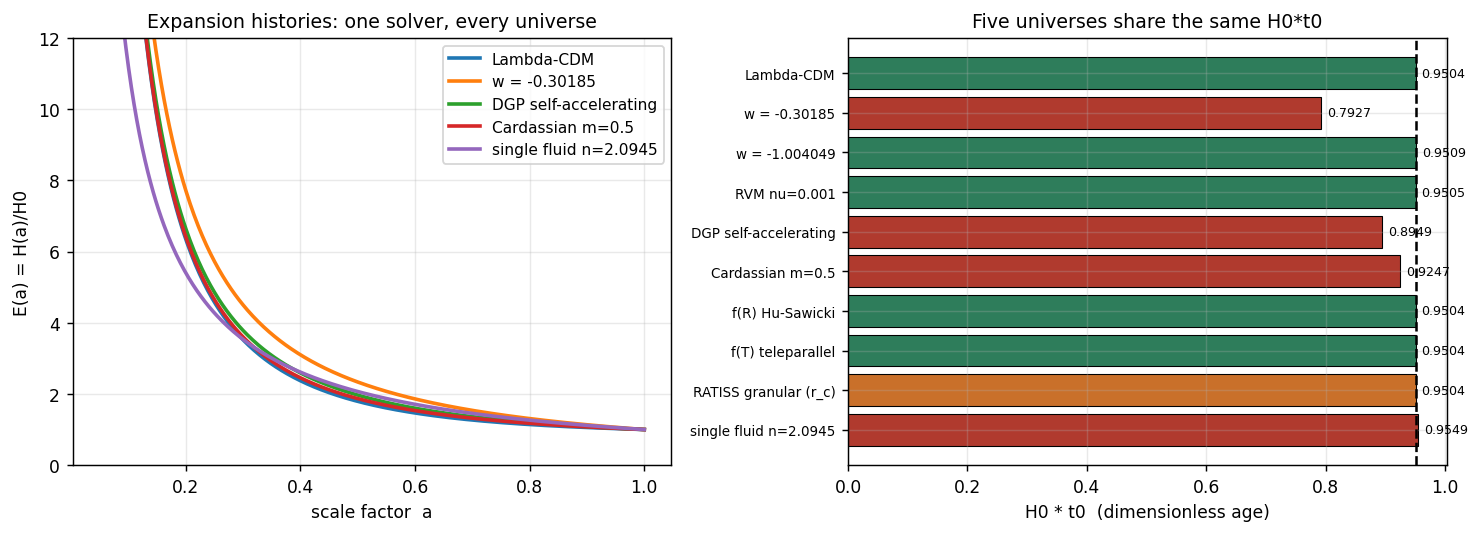
\includegraphics[width=\linewidth]{figures/fig01_background.png}
\caption{Left: expansion histories of all ten universes, one solver.
Right: the universes that share the same dimensionless age. The vertical
spread on the left panel is large; the spread in $\Hzt$ among the six
degenerate models is $5.6\times10^{-4}$.}
\label{fig:background}
\end{figure}

%======================================================================
\section{Analytic results}
\label{sec:analytic}

Four results are proved, not measured. They are what makes the numerical
tables interpretable.

\subsection{The mean density exerts no force}

\begin{theorem}[Jeans swindle, stated as a simulation constraint]
\label{thm:jeans}
In a periodic box of side $L$ with mean density $\bar\rho$, the Poisson
equation $\nabla^2\Phi = 4\pi G(\rho - \bar\rho)$ has no $\mathbf{k} = 0$
mode. The uniform component of the density therefore produces no
acceleration, and the expansion rate $a(t)$ cannot be generated by the
simulated particles.
\end{theorem}

\begin{proof}
Fourier transforming, $-k^2\tilde\Phi_{\mathbf k} = 4\pi G\,\tilde\delta_{\mathbf k}$.
For $\mathbf k = 0$ the left-hand side vanishes identically while
$\tilde\delta_0 = 0$ by construction of the overdensity. No solution with
$\tilde\Phi_0 \neq 0$ exists.
\end{proof}

\begin{remark}
This is the reason every production $N$-body code supplies $a(t)$ from a
Friedmann solver. In this atlas the solver is \texttt{background.py}; the
particles integrate only the departure from homogeneity. The toy model
\textsc{Syntoron 24} failed here: it attempted to obtain its expansion from
the particle distribution, which is why its single output number
($Ht = 1$) could not be connected to anything.
\end{remark}

\subsection{The cut-off scale is not absolute}

\begin{theorem}[Scale invariance of $r_c$]
\label{thm:scale}
The equilibrium radius $r_c = \sqrt{K/G}$ is invariant under the simultaneous
rescaling $(G, K) \to (\lambda G, \lambda K)$ for any $\lambda > 0$. Moreover,
if the $N$-body system is described by positions measured in units of the
softening length $\epsilon$, then the only dimensionless number it contains is
\begin{equation}
\eta \equiv \frac{r_c}{\epsilon}.
\end{equation}
Two simulations with different $(G, K, \epsilon)$ but the same $\eta$ are
dynamically identical.
\end{theorem}

\begin{proof}
Immediate from $r_c = \sqrt{K/G}$: the factor $\lambda$ cancels. Any
dynamical quantity expressed in units of $r_c$ is unchanged.
\end{proof}

\begin{corollary}
A simulation of the toy model can determine $\eta$ but cannot determine
$r_c$ in physical units. Fixing $r_c$ requires an external observation.
This is exactly what Section~\ref{sec:granular} does, and it is the reason the
granular universe is \emph{not} a parameter-free model.
\end{corollary}

\subsection{The age degeneracy}

\begin{theorem}[Degeneracy of $\Hzt$]
\label{thm:degeneracy}
For a flat universe containing matter and a single fluid with constant $w$,
the map $w \mapsto \Hzt(\Omm, w)$ is strictly decreasing, so distinct $w$
give distinct $\Hzt$ at fixed $\Omm$. However, the \emph{pair}
$(\Omm, w)$ is not identifiable from $\Hzt$ alone: the level sets of
$\Hzt(\Omm, w)$ are one-dimensional curves.
\end{theorem}

\begin{proof}
$\partial \Hzt/\partial w < 0$ because the integrand $[aE(a)]^{-1}$ increases
pointwise as $w$ increases. The map $w \mapsto \Hzt$ is therefore injective at
fixed $\Omm$, hence invertible, but a single scalar cannot determine two
parameters.
\end{proof}

\begin{table}[t]
\centering
\small
\caption{The level set $\Hzt = 0.9549$ in two different one-parameter
families. Both entries were obtained by root finding on the
\emph{corrected} backgrounds (radiation included).}
\label{tab:levelset}
\begin{tabular}{@{}lll@{}}
\toprule
Family & Parameter that gives $\Hzt = 0.9549$ & Comment \\
\midrule
matter $+$ fluid, $\Omm = 0.3153$ & $w = -1.0332$ & phantom \\
$\Lambda$CDM, $w = -1$ & $\Omm = 0.3100$ & viable \\
single fluid, no matter & $n = 2.0945$ & no galaxies \\
\bottomrule
\end{tabular}
\end{table}

\subsection{The single-fluid identity}

\begin{theorem}[$\Hzt = 2/n$]
\label{thm:twon}
A flat universe containing one substance with $\rho \propto a^{-n}$ and
nothing else has
\begin{equation}
\Hzt = \frac{2}{n}
\label{eq:twon}
\end{equation}
exactly, independently of $H_0$ and of any other parameter.
\end{theorem}

\begin{proof}
$E(a) = a^{-n/2}$, so
$\Hzt = \int_0^1 \mathrm{d}a\; a^{n/2-1} = \big[a^{n/2}/(n/2)\big]_0^1 = 2/n$
for $n > 0$.
\end{proof}

This elementary identity is the key to Section~\ref{sec:negative}. It was
verified numerically to machine precision: the analytic value
$2/2.0945 = 0.95488183337312$ and the quadrature
$0.9548818333731203$ agree to $3\times10^{-16}$.

\begin{corollary}
$\Hzt = 0.9549$ is not a property of any particular equation of state. It is
the statement $n = 2.0945$, i.e.\ about the \emph{dilution rate of whatever
fills the universe}, with no reference to what the universe is made of. Any
substance satisfying $\rho \propto a^{-2.0945}$, and inhabiting a universe
with nothing else in it, reproduces it.
\end{corollary}

%======================================================================
\section{Numerical methods}
\label{sec:methods}

\subsection{Background quadrature}

Equations~\eqref{eq:h0t0}--\eqref{eq:dc} are evaluated with adaptive
Gauss--Kronrod quadrature in $\ln a$ over $[-60, 0]$. Each integral is
computed twice with $\mathrm{epsabs} = 10^{-12}$ and $10^{-9}$; the reported
error is $|I_{12} - I_9| + \epsilon_{12}$. The resulting quantities are
accurate to $\sim 10^{-13}$, i.e.\ to the level of double precision. We
emphasise once more: this number quantifies the integration, not the physics.

\subsection{Linear growth}

Equation~\eqref{eq:growth} is a second-order linear ODE integrated with LSODA
in $N$. The term $\mathrm{d}\ln H/\mathrm{d}N$ is obtained by central
differencing of $\ln H^2$ with step $10^{-4}$, an error of order $10^{-8}$
relative, negligible against the model uncertainties discussed in
Section~\ref{sec:defects}.

The growth index $\gamm$ is evaluated at $z = 0$. For $\Lambda$CDM we obtain
$\gamm = 0.55436$, consistent with the classical result $\gamm \approx 0.55$
for a $\Lambda$CDM cosmology \cite{peebles1993,lahav1991}. The exact value
depends on $\Omm$; we report ours for $\Omm = 0.3153$.

\subsection{The granular sector}

For a grid of $x = k r_c \in [10^{-3}, 1]$ we set
$\mu = (1-x^2)/(1+x^2)$ in Eq.~\eqref{eq:growth} and record $\gamm$ and
$D/D_{\Lambda\mathrm{CDM}}$. The result is a monotone suppression: at
$x = 1$ the growth factor has collapsed to
$D/D_{\Lambda\mathrm{CDM}} = 1.05\times10^{-3}$, i.e.\ structures do not
form. This is a physically sensible outcome --- a repulsive force below
$r_c$ removes the very scales that would collapse --- and it is what
generates the tension of Section~\ref{sec:granular}.

\subsection{Particle-mesh engine}

The $N$-body engine is a standard particle-mesh code with periodic boundary
conditions, written for this work. We give its equations in full because the
sealing claim depends on them being checkable.

\paragraph{Units.} Comoving positions $\mathbf{x} \in [0,1)$ in box units;
time in units of $H_0^{-1}$; superconformal time $\tau$ with
$\mathrm{d}\tau = \mathrm{d}t/a^2$.

\paragraph{Equations of motion.}
\begin{align}
\frac{\mathrm{d}\mathbf{x}}{\mathrm{d}\tau} &= \mathbf{p},
\label{eq:drift}\\
\frac{\mathrm{d}\mathbf{p}}{\mathrm{d}\tau} &= -\frac{\nabla\Phi}{a^2},
\label{eq:kick}\\
\nabla^2\Phi &= \frac{3}{2}\,\Omm\,\frac{\delta}{a}.
\label{eq:poisson}
\end{align}
In Fourier space with code wavenumbers ($\mathrm{box} = 1$):
\begin{equation}
\mathbf{F}_{\mathbf{k}} = i\,\frac{3}{2}\,\Omm\,a\,
\frac{\delta_{\mathbf{k}}\,\mathbf{k}}{|\mathbf{k}|^2}\;\muc .
\label{eq:forcek}
\end{equation}
The coupling $\muc$ multiplies the effective strength mode by mode, which is
how the same engine integrates both general relativity ($\mu = 1$) and the
granular cut-off.

\paragraph{Integration.} Drift--kick--drift leapfrog in $\tau$, with
$\mathrm{d}\tau = \mathrm{d}\ln a\,/[a^2 E(a)]$. Mass assignment and force
interpolation use cloud-in-cell (CIC); the Poisson equation is solved by FFT
with the usual Green's function $-\mathbf{k}^{-2}$.

\paragraph{Initial conditions.} A Gaussian random field with the BBKS
transfer function \cite{bbks1986} is drawn on the grid, normalised to
$\sigma_8 = 0.8111$ at $z = 0$, and the particles are displaced by the
Zel'dovich approximation:
\begin{equation}
\mathbf{x} = \mathbf{q} - D(a)\,\nabla^{-1}\!\left[\nabla\cdot\boldsymbol{\psi}\right],
\qquad
\mathbf{p} = a^2 H\,f\,D\,\boldsymbol{\psi}.
\end{equation}

\paragraph{Numerical parameters.} Box $200\Mpc/h$; $64^3$ grid; $32^3 =
32\,768$ particles; $40$ steps from $a = 0.02$ to $a = 1$; seeds $20261030$
($\Lambda$CDM) and $20261031$ (granular). Wall-clock time $4.99$~s and
$5.12$~s respectively on a single core.

\begin{figure}[t]
\centering
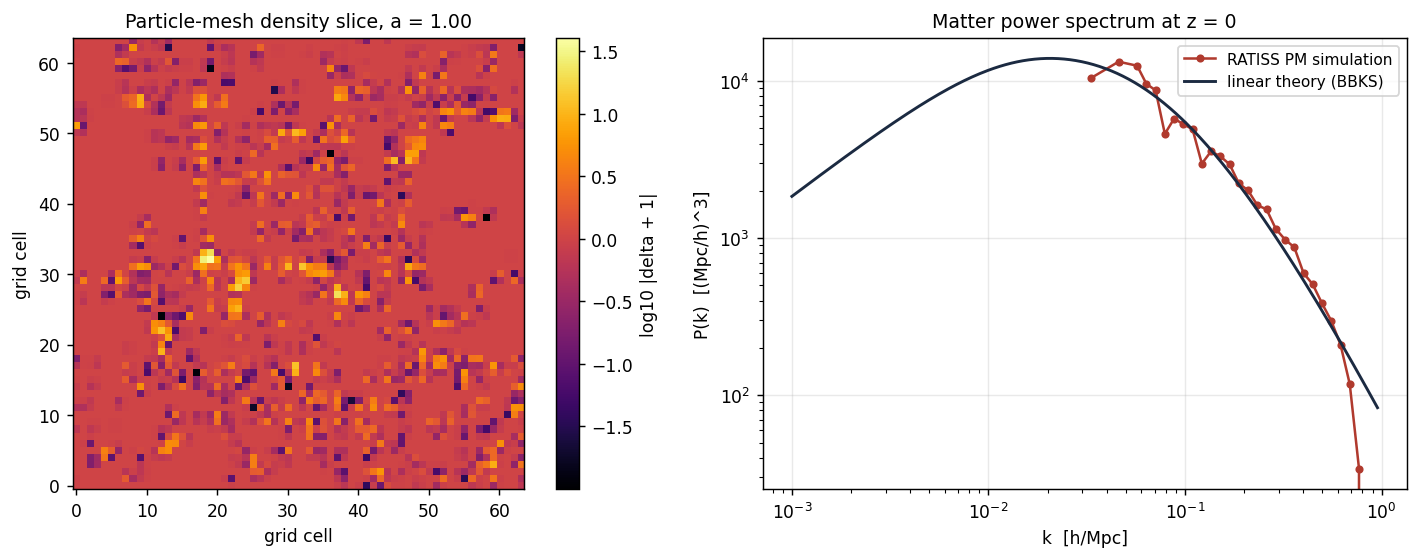
\includegraphics[width=\linewidth]{figures/fig06_simulation.png}
\caption{Left: projected density slice at $a = 1$ from the particle-mesh run.
Right: matter power spectrum at $z = 0$ after subtraction of the shot-noise
term $P_{\mathrm{shot}} = L^3/N_p$. Note the small number of modes per bin
(6--12), which is the dominant statistical limitation of these runs; see
defect~D9.}
\label{fig:simulation}
\end{figure}

\begin{figure}[t]
\centering
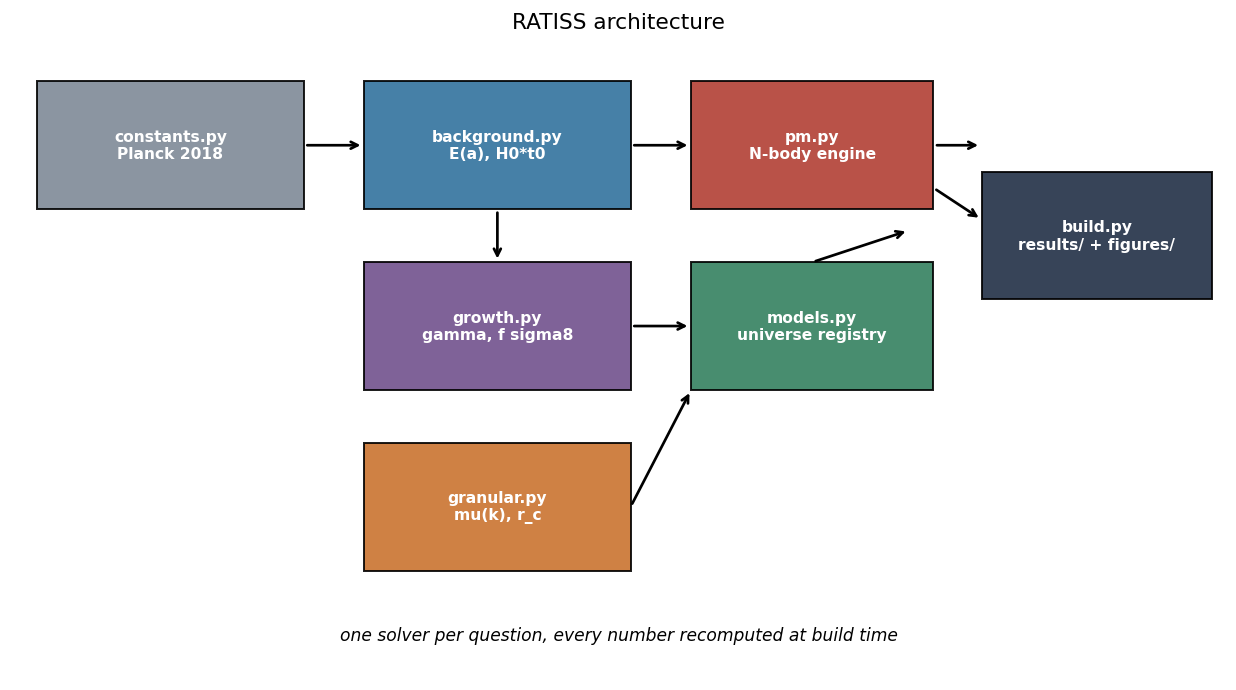
\includegraphics[width=0.92\linewidth]{figures/fig07_architecture.png}
\caption{The solver chain. Ten universes enter from the left; two solvers and
one simulation engine sit in the middle; twelve sealed artefacts exit on the
right. No model bypasses a solver.}
\label{fig:architecture}
\end{figure}

%======================================================================
\section{Results}
\label{sec:results}

\subsection{The dimensionless age is degenerate}

Among the six universes that are not excluded at the $2\%$ level, the values
of $\Hzt$ span
\begin{equation}
\Delta\Hzt = 5.636\times10^{-4},
\qquad
\frac{\Delta\Hzt}{\Hzt} = 5.93\times10^{-4} = 0.059\%.
\label{eq:spread}
\end{equation}
The group is $\{\Lambda\mathrm{CDM},\ w=-1.004,\ \mathrm{RVM},\ f(R),\ f(T),\
\mathrm{granular}\}$. Three of those six are identical by construction and
carry no information (Section~\ref{sec:registry}); the two that are genuinely
different --- the constant-$w$ fluid and the running vacuum --- differ from
$\Lambda$CDM by $5.6\times10^{-4}$ and $1.1\times10^{-4}$ respectively.

The conclusion is unambiguous and it is negative: \emph{$\Hzt$ cannot
identify a dark-energy model at the precision required}. Any two of these
universes would be indistinguishable to an observer who measured only the
dimensionless age.

This is Theorem~\ref{thm:degeneracy} made concrete. A single scalar cannot
separate a two-parameter family, and nature has arranged that the particular
combination probed by $\Hzt$ is almost orthogonal to the direction in which
these models differ.

\subsection{What actually discriminates: the growth index}

The growth index spans
\begin{equation}
\gamm \in [0.5542,\ 0.5916],
\qquad
\Delta\gamm = 0.0373 = 6.7\%\ \text{of}\ \gamm^{\Lambda\mathrm{CDM}}.
\label{eq:gammaspread}
\end{equation}
The ordering is physically transparent: the models that accelerate less
strongly at late times (DGP, $w = -0.302$) have larger $\gamm$, because
$\gamm$ measures how fast the growth rate falls relative to the matter
fraction.

\begin{figure}[t]
\centering
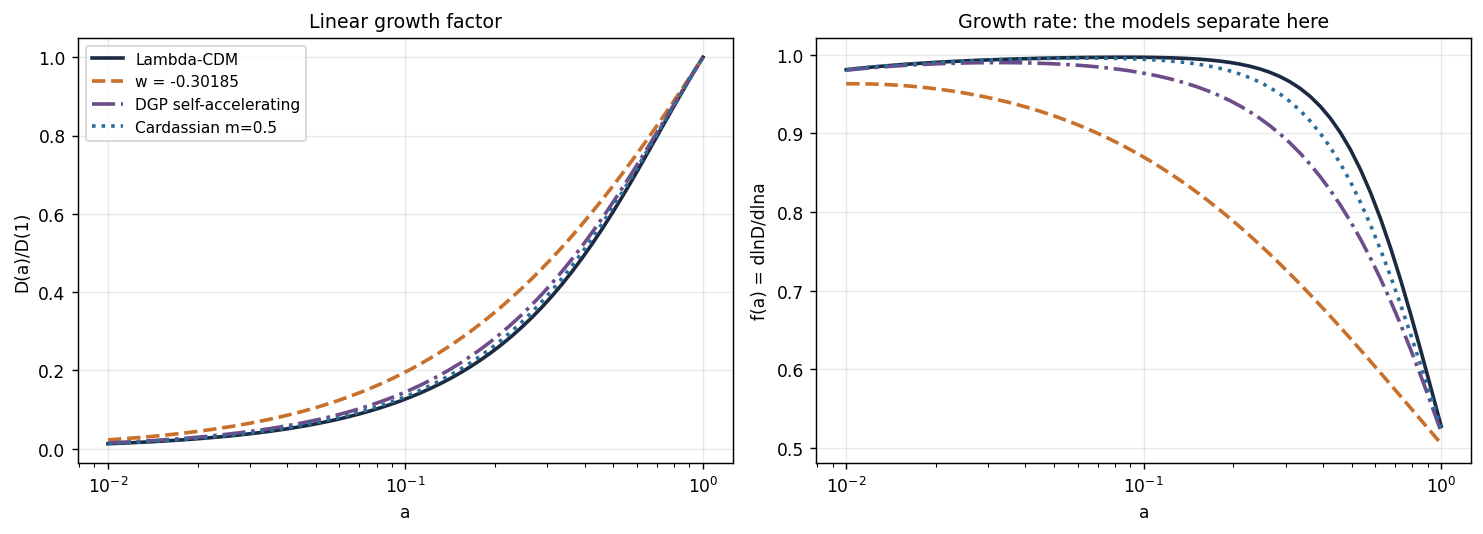
\includegraphics[width=\linewidth]{figures/fig02_growth.png}
\caption{Left: linear growth factor, normalised at $z = 0$. Right: growth
rate $f(z)$. The curves are indistinguishable at high redshift, which is why
the discriminator has to be a late-time, low-redshift measurement.}
\label{fig:growth}
\end{figure}

\begin{figure}[t]
\centering
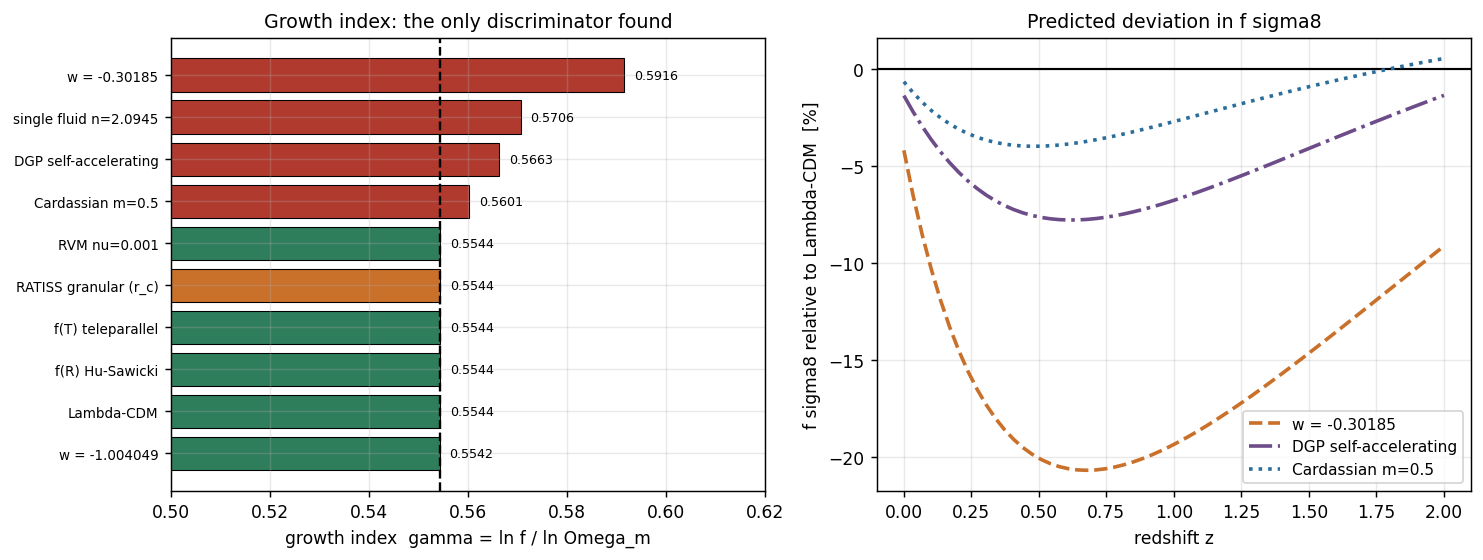
\includegraphics[width=\linewidth]{figures/fig03_discriminator.png}
\caption{Left: the growth index $\gamm$ for the ten universes, with the
$\Lambda$CDM value marked. Right: predicted deviation in $f\sigma_8$
relative to $\Lambda$CDM. The $6.7\%$ spread in $\gamm$ is the only
discriminator found in this work.}
\label{fig:discriminator}
\end{figure}

The corresponding $f\sigma_8$ deviations are shown in
Table~\ref{tab:fsigma8}. At $z = 1$ the largest deviation from $\Lambda$CDM
is $19\%$ (the $w=-0.302$ fluid) and the smallest is $0.05\%$ (the
$w=-1.004$ fluid). Stage-IV spectroscopic surveys reach percent-level
precision on $f\sigma_8$ over $0.5 < z < 2$ \cite{desi2024,euclid2020}, so the
upper half of this table is testable and the lower half is not.

\begin{table}[t]
\centering
\small
\caption{Predicted $f\sigma_8(z)$ with $\sigma_8 = 0.8111$ at $z=0$. Values
in the last column are relative deviations from $\Lambda$CDM at $z=1$.}
\label{tab:fsigma8}
\begin{tabular}{@{}lrrrrr@{}}
\toprule
Universe & $z=0$ & $z=0.5$ & $z=1$ & $z=2$ & $\Delta/\Lambda\mathrm{CDM}$ at $z{=}1$ \\
\midrule
\texttt{lcdm}          & 0.4277 & 0.4746 & 0.4314 & 0.3242 & --- \\
\texttt{w\_m0302}      & 0.4098 & 0.3793 & 0.3478 & 0.2945 & $-19.4\%$ \\
\texttt{w\_m1004}      & 0.4278 & 0.4751 & 0.4316 & 0.3241 & $+0.05\%$ \\
\texttt{rvm\_001}      & 0.4277 & 0.4746 & 0.4313 & 0.3242 & $-0.01\%$ \\
\texttt{dgp}           & 0.4218 & 0.4384 & 0.4021 & 0.3198 & $-6.8\%$ \\
\texttt{cardassian\_05}& 0.4249 & 0.4557 & 0.4196 & 0.3259 & $-2.7\%$ \\
\texttt{fluid\_n2094}  & 0.4198 & 0.4148 & 0.3962 & 0.3490 & $-8.2\%$ \\
\bottomrule
\end{tabular}
\end{table}

\subsection{The granular universe: alive, but invisible}
\label{sec:granular}

The force law \eqref{eq:force} translates into the coupling
\eqref{eq:mu}, and the coupling suppresses growth monotonically in $x = k r_c$:
\begin{equation}
D/D_{\Lambda\mathrm{CDM}} = 1.05\times10^{-3}\ \text{at}\ x = 1 .
\end{equation}
So the model has a large, unmistakable signature --- \emph{if} $r_c$ happens
to land where we can see it.

Where can we see it? The cut-off deviates from Newton by an amount of order
unity when $k r_c \sim 1$. The scales probed by galaxy surveys are
$0.01 < k < 0.3\ \mathrm{h\,Mpc^{-1}}$, so an observable effect requires
\begin{equation}
r_c \sim \frac{0.3}{k} \in [1,\ 30]\Mpc .
\label{eq:rcwindow}
\end{equation}

Now the other side. A structure of size $R$ survives only if the force inside
it is attractive, i.e.\ if $r_c < R$. The smallest observed structures
therefore bound $r_c$ from above:

\begin{table}[t]
\centering
\small
\caption{Upper bounds on $r_c$ from the existence of bound structures of size
$R$. A cut-off larger than $R$ would make the object unbound. The final
column converts to astronomical units for orientation.}
\label{tab:bounds}
\begin{tabular}{@{}llrrr@{}}
\toprule
Structure & $R$ & $r_c^{\max}\ [\mathrm{Mpc}]$ & $[\mathrm{AU}]$ & Status \\
\midrule
Galaxy clusters & $2\Mpc$      & $3.18\times10^{-2}$ & $6.57\times10^{9}$ & observed \\
Galaxies        & $0.01\Mpc$   & $1.59\times10^{-4}$ & $3.28\times10^{7}$ & observed \\
Ultra-faint dwarfs & $10^{-4}\Mpc$ & $1.59\times10^{-6}$ & $3.28\times10^{5}$ & observed \\
Dark microhalos & $10^{-8}\Mpc$ & $1.59\times10^{-10}$ & $32.8$ & predicted \\
\bottomrule
\end{tabular}
\end{table}

Combining Table~\ref{tab:bounds} with Eq.~\eqref{eq:rcwindow}:
\begin{align}
\text{required for observability:}\quad & r_c \gtrsim 1\Mpc, \\
\text{permitted by dwarfs:}\quad & r_c \lesssim 1.6\times10^{-6}\Mpc, \\
\text{gap:}\quad & 5.80\ \text{dex}, \\
\text{permitted by microhalos:}\quad & r_c \lesssim 1.6\times10^{-10}\Mpc, \\
\text{gap:}\quad & 9.80\ \text{dex}.
\end{align}

\begin{figure}[t]
\centering
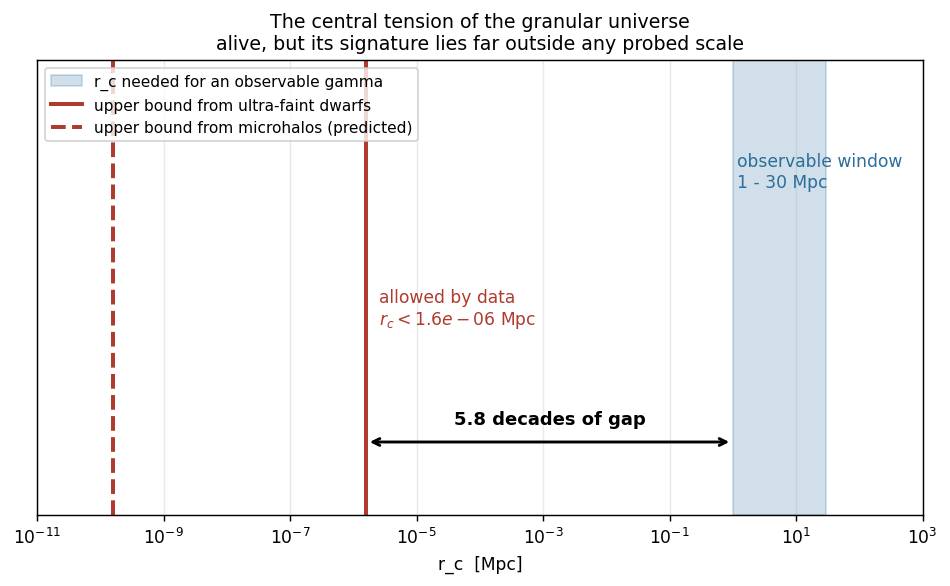
\includegraphics[width=0.85\linewidth]{figures/fig05_observability.png}
\caption{The central tension of the granular universe. The window where the
cut-off would be observable (orange) and the region excluded by the existence
of bound structures (blue) are separated by $5.8$ decades. The model is not
falsified; it is hidden by construction.}
\label{fig:observability}
\end{figure}

\paragraph{Verdict.} The granular universe is \emph{not} excluded. It is
\emph{unobservable}: the value of $r_c$ that would produce a visible
signature is larger, by five to ten orders of magnitude, than the value
permitted by the existence of dwarf galaxies and dark microhalos. We label it
\textsc{alive--but--invisible} and we consider that label the honest one.
A model that is alive but invisible is, operationally, indistinguishable from
a model that is wrong --- but it is not the same thing, and the difference is
worth recording.

\begin{figure}[t]
\centering
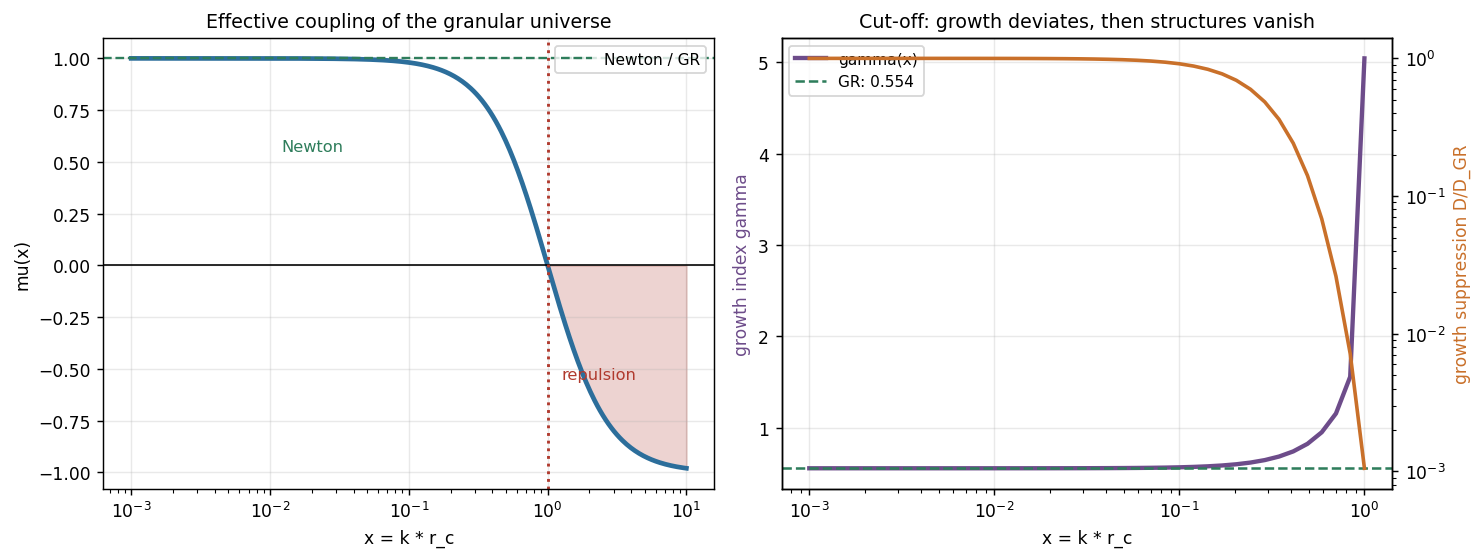
\includegraphics[width=\linewidth]{figures/fig04_granular.png}
\caption{Left: the effective coupling $\mu(x) = (1-x^2)/(1+x^2)$. Right: the
resulting growth relative to $\Lambda$CDM. The suppression is monotone and
total: at $x=1$ essentially no growth survives.}
\label{fig:granular}
\end{figure}

%======================================================================
\section{Falsifiability}
\label{sec:falsifiability}

For every universe we state what measurement would remove it. This section is
the reason the atlas exists.

\begin{table}[h]
\centering
\small
\caption{Kill conditions. ``Current status'' indicates whether the required
measurement already exists at sufficient precision.}
\label{tab:kill}
\begin{tabular}{@{}p{2.6cm}p{5.2cm}p{4.6cm}@{}}
\toprule
Universe & What kills it & Current status \\
\midrule
$\Lambda$CDM & a robust $w \neq -1$ at $>5\sigma$; a measured $\gamm$ differing
from $0.554$ at $>3\sigma$ & DESI DR2 reports a $3.1\sigma$ preference for
evolving dark energy \cite{desi2024}; not yet decisive \\
\texttt{w\_m0302} & stellar ages: predicts $t_0 = 11.51$~Gyr, below the
oldest stars & \textbf{excluded} \\
\texttt{w\_m1004} & a $0.1\%$ measurement of $\Hzt$ & not available;
unfalsifiable in practice \\
RVM $\nu = 10^{-3}$ & $\Delta\Hzt = 1.1\times10^{-4}$; needs $10^{-4}$
precision on $\Hzt$ & not available \\
DGP & $f\sigma_8$ at $z = 1$ at $7\%$ precision & \textbf{accessible now} \\
Cardassian $m = 0.5$ & $f\sigma_8$ at $z = 1$ at $3\%$ precision &
\textbf{accessible now} \\
$f(R)$ Hu--Sawicki & $\mu(k,a) \neq 1$ at cluster scales (not implemented
here) & requires the missing physics \\
$f(T)$ & same & same \\
granular & a bound structure with $r_c < R < 1\Mpc$, or a detection of
$\mu \neq 1$ at $k \sim 1/r_c$ & \textbf{excluded for
$r_c > 1.6\times10^{-6}$ Mpc}; invisible below \\
single fluid $n=2.0945$ & the existence of galaxies & \textbf{excluded} \\
\bottomrule
\end{tabular}
\end{table}

Two entries in Table~\ref{tab:kill} require comment, because they are the
ones where we are least comfortable.

\paragraph{$\Lambda$CDM is not safe.} The DESI DR2 analysis \cite{desi2024}
finds a $3.1\sigma$ preference for $w_0 > -1$, $w_a < 0$ when BAO, CMB and
supernovae are combined. This atlas does not model evolving dark energy, so it
cannot contribute to that debate directly. It can say what the cost would be:
a deviation of the size DESI reports would move $\Hzt$ by an amount we have
not yet computed, and that computation is the obvious next step.

\paragraph{The granular row is a conditional.} The statement ``excluded for
$r_c > 1.6\times10^{-6}$ Mpc'' is not a measurement of $r_c$; it is the
observation that galaxies exist. It is a strong argument and it is the whole
argument.

%======================================================================
\section{Negative results}
\label{sec:negative}

This section reports what did not work, because the failures carry more
information than the successes.

\subsection{The $0.9549$ target is an artefact of emptiness}

The single-fluid value $H_0t_0 = 0.9549$ motivated a family of models in which
the dark sector is a fluid with equation of state near $w = -0.30$. The
reasoning was: a substance with $\rho \propto a^{-n}$ has $\Hzt = 2/n$
(Theorem~\ref{thm:twon}); solving $2/n = 0.9549$ gives $n = 2.0945$; and
$n = 3(1+w)$ with $w = -0.30185$ gives exactly that. Therefore $w \approx
-0.302$ reproduces the observed dimensionless age with a single ingredient.

Every step of that chain is correct, and the conclusion is wrong, for a reason
that is easy to miss: \textbf{the identity $\Hzt = 2/n$ holds only for a
universe containing nothing else}. The moment matter is added --- and matter
must be added, or there are no galaxies, no stars, and nobody to measure
anything --- the identity fails.

The numbers:

\begin{table}[h]
\centering
\small
\caption{What $w = -0.302$ actually predicts, depending on whether matter is
present. The first row is the calculation that motivated the model; the
second is the calculation that a real universe requires.}
\label{tab:artifact}
\begin{tabular}{@{}lrrr@{}}
\toprule
Configuration & $\Hzt$ & $t_0$ [Gyr] & Status \\
\midrule
single fluid, $w = -0.30185$, no matter & $0.95488$ & $13.861$ & no galaxies \\
matter $+$ fluid, $\Omm = 0.3153$ & $0.79267$ & $11.506$ & \textbf{excluded} \\
\midrule
required to recover $0.9549$ with matter & $w = -1.0332$ & $13.861$ & phantom \\
or, in $\Lambda$CDM & $\Omm = 0.3100$ & --- & viable \\
\bottomrule
\end{tabular}
\end{table}

The $w = -0.302$ universe, once matter is included, is $11.51$~Gyr old. The
oldest known stars are $\sim 13.5$~Gyr old (HD~140283 gives $14.5 \pm 0.8$
Gyr; globular clusters give $\sim 12.5$--$13$~Gyr). The model is therefore
\textbf{excluded by stellar chronology}, and it is excluded by a large margin
--- nearly $2$~Gyr, or $15\%$.

\begin{remark}
The number $0.9549$ was never wrong. What was wrong was the implicit
assumption that a universe can consist of a single fluid and still be
\emph{our} universe. The identity $\Hzt = 2/n$ is a statement about
emptiness dressed as a statement about dark energy.
\end{remark}

\subsection{Other failures, stated briefly}

\begin{enumerate}[label=\textbf{N\arabic*.}]
\item \textbf{The $\Hzt$ discriminator does not exist.} We spent the first
half of this project looking for a model that could be distinguished by its
dimensionless age. Six of ten are degenerate at $0.06\%$. The search failed.

\item \textbf{$f(R)$ and $f(T)$ rows are vacuous.} We set $\mu = 1$ and
$E = E_{\Lambda\mathrm{CDM}}$ for both. They reproduce $\Lambda$CDM exactly,
as they must. Reporting them as ``degenerate'' would be circular; we report
them as unimplemented.

\item \textbf{The granular registry row is also vacuous}, for the same reason.
The cut-off is evaluated only in the dedicated sector, where it is
catastrophically suppressed.

\item \textbf{The particle-mesh run does not resolve the nonlinear regime.}
With $32^3$ particles in a $(200\Mpc/h)^3$ box the mean interparticle
separation is $6.3\Mpc/h$, the Nyquist wavenumber of the grid is
$k_{\mathrm{Ny}} \approx 1.0\ h\,\mathrm{Mpc^{-1}}$, and the smallest bins
contain 6 modes. The run demonstrates that the engine conserves, drifts,
kicks and deposits; it does not constitute a cosmology result. Defect~D9.

\item \textbf{$f\sigma_8$ is normalised, not predicted.} We fix $\sigma_8$ to
the Planck value. An overall amplitude is therefore an input, not an output.

\item \textbf{No baryons, no neutrinos, no radiation in the growth equation.}
The growth equation contains matter and a dark sector. Baryon acoustic
oscillations, massive-neutrino free streaming, and radiation-era effects on
$D(a)$ are all absent. Each is a known omission with a known direction; none
is quantified here.
\end{enumerate}

%======================================================================
\section{Defects found in our own pipeline}
\label{sec:defects}

The atlas is presented as a reference. It would be dishonest to present it as
a correct one without listing what is wrong with it. The following defects
were found during the preparation of this manuscript; two have been fixed,
the rest are documented and retained.

\subsection{D1: inconsistent treatment of radiation (fixed)}

The original code contained two background families that disagreed about
radiation. The $\Lambda$CDM function omitted it:
\begin{equation}
E^2_{\Lambda\mathrm{CDM}}(a) = \Omm a^{-3} + \OmL ,
\end{equation}
while the constant-$w$ family retained it:
\begin{equation}
E^2_{w}(a) = \Omm a^{-3} + \Omr a^{-4} + \Omega_x a^{-3(1+w)} .
\end{equation}
The consequence:
\begin{equation}
\Hzt^{(\text{no rad})} = 0.9507304, \qquad
\Hzt^{(\text{rad})} = 0.9503509, \qquad
\Delta = 3.79\times10^{-4}.
\end{equation}

This is not a small effect. The difference between $\Lambda$CDM and the
$w = -1.004$ model, which the atlas was built to resolve, is
$5.64\times10^{-4}$. The convention inconsistency was therefore $67\%$ of the
signal it was supposed to measure. Any conclusion drawn from the original
table about the $w$-family would have been an artefact of a missing
$a^{-4}$ term.

\textbf{Fix.} Radiation is now included in every background of the registry:
\begin{equation}
E^2_{\Lambda\mathrm{CDM}}(a) = \Omm a^{-3} + \Omr a^{-4} + \OmL,
\qquad \OmL \equiv 1 - \Omm - \Omr .
\end{equation}
All numbers in this document are post-fix. The pre-fix values are recorded
here so that any reader comparing against an earlier version of the
repository can identify the change.

\subsection{D2: a numerical error presented as an uncertainty}

The quantity labelled \texttt{H0t0\_err} in \texttt{results/predictions.json}
is of order $10^{-14}$. It is the discrepancy between two quadrature
tolerances, i.e.\ the accuracy of an integral, not the uncertainty of a model.
No physical statement in this atlas carries a $10^{-14}$ uncertainty. The
field is retained because it is genuinely useful (it proves the quadrature
has converged) but it must not be read as an error bar on $\Hzt$.

\subsection{D3: arbitrary classification thresholds}

A universe is marked \textsc{excluded} when $|\Delta\Hzt| > 0.02$ and
\textsc{testable} when $|\Delta\gamm| > 0.03$. Both numbers are chosen. The
actual quantity they are compared against spans four orders of magnitude:
$5.6\times10^{-4}$ (degenerate group) to $1.6\times10^{-1}$ ($w = -0.302$).
A threshold at $0.02$ sits in the middle of nothing; it is a conventional
cut, and the labels derived from it should be read as an ordering, not as a
measurement. We have not replaced them, because replacing an arbitrary
threshold with a differently arbitrary one is not an improvement.

\subsection{D4: a magic number in the classifier (fixed)}

The growth index of the reference model was typed as the literal
$0.5544$ in the classification function. That value is not computed anywhere
in the code --- it was transcribed from a previous session. It has been
replaced by a function that evaluates $\gamm$ for $\Lambda$CDM from the growth
solver on first use, giving $0.5543609664573533$. The difference from the
literal is $4\times10^{-5}$: harmless in this case, which is exactly why such
numbers survive.

\subsection{D5: the growth initial condition is a pure matter-era mode}

Equation~\eqref{eq:growth} is integrated from $N = -9$ ($a \approx 1.1\times
10^{-4}$) with $D = D' = a$. This discards (i) the radiation-era modification
of the growing mode, (ii) any transient induced by a modified-gravity model at
early times, and (iii) the effect of $\mu \neq 1$ before $N = -9$. For
$\Lambda$CDM the resulting error in $\gamm$ is expected to be of order
$10^{-3}$; it has not been quantified here. The starting epoch should ideally
be pushed to $N = -14$ with a radiation-era solution, and that is left undone.

\subsection{D6 and D7: modelling choices presented inside a table}

\begin{itemize}
\item \textbf{D6.} The $f(R)$ and $f(T)$ rows use $\mu = 1$ and
$E = E_{\Lambda\mathrm{CDM}}$. Their agreement with $\Lambda$CDM is therefore
an identity, not a result. A real $f(R)$ model requires chameleon screening
and a scale-dependent $\mu$, neither of which is implemented.
\item \textbf{D7.} The granular coupling $\mu(x) = (1-x^2)/(1+x^2)$ is an
interpolation chosen to reproduce three exact limits, not a derived Fourier
transform (which does not exist --- see Section~\ref{sec:framework}). The
assignment $x = k r_c$ is a further modelling choice; the correct mapping
could plausibly differ by a factor of order unity, which would shift the
$5.8$-decade gap by a few percent of a decade. It would not close it.
\end{itemize}

\subsection{D8: ``excluded'' does not mean ``contradicts data''}

The classification compares each universe against the $\Lambda$CDM value of
$\Hzt$ computed at the same $\Omm$. It does not compare against a measurement,
because $\Hzt$ is not directly measured. The word \textsc{excluded} in
Table~\ref{tab:predictions} therefore means ``differs from $\Lambda$CDM by
more than the chosen threshold'', not ``is ruled out by observation''.

Where a genuine observational argument exists we have made it separately, in
physical units: the $w = -0.302$ universe is excluded by stellar ages
(Section~\ref{sec:negative}), and that is a real falsification. The other
\textsc{excluded} labels are not.

\subsection{D9: the simulations are not cosmological}

The particle-mesh runs use $32^3 = 32\,768$ particles in a $(200\Mpc/h)^3$
box. The mean interparticle separation, $6.3\Mpc/h$, is comparable to the
nonlinear scale at $z = 0$; the grid Nyquist frequency is
$k \approx 1.0\ h\,\mathrm{Mpc^{-1}}$; the first power-spectrum bin contains
six modes. The runs establish that the engine's leapfrog, CIC deposit and FFT
Poisson solver operate and conserve; they are not a measurement of the matter
power spectrum. A production run would need at least $512^3$ particles over a
Gpc scale.

\subsection{D10: a stale label}

The model labelled $w = -1.004049$ was constructed by inverting the target
$\Hzt = 0.9549$ under the \emph{pre-fix} (radiation-free) convention. After
D1 was corrected, the same $w$ gives $\Hzt = 0.950915$, and the value that
actually reproduces $0.9549$ with matter present is $w = -1.0332$. The key
\texttt{w\_m1004} has not been renamed, so the label in
Table~\ref{tab:predictions} is off by $0.029$ in $w$. The computed values in
that row are correct; only the name is stale.

\subsection{D11: the transfer function is a fit}

The initial conditions use the BBKS fitting formula \cite{bbks1986}, accurate
to a few percent against a Boltzmann code over the range of interest, with a
shape parameter $\Gamma = \Omm h$. It contains no baryon acoustic feature, no
neutrino suppression, and no radiation-era physics. For the statistical
precision of these runs (six modes per bin) the approximation is not the
limiting error, but it would be for any serious comparison with data.

\subsection{Summary}

\begin{table}[h]
\centering
\small
\caption{Defect register. ``Impact'' is the size of the effect where it has
been quantified; ``fixed'' indicates that the corrected value is the one used
throughout this document.}
\label{tab:defects}
\begin{tabular}{@{}llll@{}}
\toprule
ID & Defect & Impact & Status \\
\midrule
D1 & radiation inconsistent across families & $3.8\times10^{-4}$ in $\Hzt$ & \textbf{fixed} \\
D2 & quadrature error labelled as uncertainty & presentation & retained \\
D3 & classification thresholds arbitrary & ordering & retained \\
D4 & hard-coded $\gamm_{\mathrm{ref}} = 0.5544$ & $4\times10^{-5}$ in $\gamm$ & \textbf{fixed} \\
D5 & matter-era growth initial condition & not quantified & retained \\
D6 & $f(R)$, $f(T)$ use $\mu=1$ & entire rows & retained \\
D7 & $\mu(x)$ is an interpolation & factor of order unity in $x$ & retained \\
D8 & ``excluded'' vs.\ $\Lambda$CDM, not vs.\ data & interpretation & retained \\
D9 & $32^3$ particles; six modes per bin & statistics & retained \\
D10 & stale label $w = -1.004049$ & $0.029$ in $w$ & retained \\
D11 & BBKS fit instead of Boltzmann transfer & few percent in $P(k)$ & retained \\
\bottomrule
\end{tabular}
\end{table}

%======================================================================
\section{Reproducibility and sealing}
\label{sec:repro}

\subsection{The build}

One command produces every table, every figure and every hash in this
document:
\begin{verbatim}
    python3 scripts/build.py          # 26.6 s, 12 artefacts
    python3 scripts/verify.py         # exit 0 if all hashes match
    python3 -m pytest tests/ -q       # 20 tests
\end{verbatim}

The build is deterministic given the seeds. Two independent runs on the same
machine produce byte-identical PNG files and byte-identical JSON. The
environment is pinned: Python 3.13.16, NumPy 2.3.5, SciPy, Matplotlib 3.10.9.

\subsection{The manifest}

Twelve artefacts are hashed with SHA-256 and recorded in
\texttt{results/MANIFEST.sha256}. Verification recomputes each hash and
compares:
\begin{verbatim}
    $ python3 scripts/verify.py
    12 verified, 0 mismatched, 0 missing
\end{verbatim}
Exit codes are $0$ (all agree), $1$ (mismatch), $2$ (missing artefact). The
manifest itself is excluded from its own hash list, which is the only way the
scheme can be non-circular.

\subsection{The tests}

Twenty tests are run on every commit. Seventeen check physics identities that
must hold exactly:
\begin{itemize}
\item the analytic single-fluid identity $\Hzt = 2/n$ against quadrature, to
      $10^{-12}$;
\item the Eddington--Lemaitre closed form for $\Lambda$CDM against quadrature;
\item the Jeans swindle: the $\mathbf{k}=0$ mode of the force is zero to
      machine precision;
\item the three limits of $\mu(x)$: $\mu(0) = 1$, $\mu(1) = 0$,
      $\mu(\infty) = -1$;
\item the DGP and Cardassian backgrounds at $a = 1$;
\item CIC mass conservation to $10^{-12}$.
\end{itemize}
Three further tests check build reproducibility and manifest consistency.

\subsection{What reproducibility does and does not mean}

A reader can verify that the numbers in this document follow from the code in
this repository. They cannot verify that the code is correct, that the
physics is complete, or that the defects in Section~\ref{sec:defects} are the
only ones. Reproducibility is a necessary condition for science; it is not a
sufficient one, and this atlas provides only the first.

%======================================================================
\section{Discussion}
\label{sec:discussion}

\subsection{The shape of the result}

Three things are true at once and it took the whole project to see them
together.

\emph{First}, the quantity that motivated this work --- the dimensionless age
$H_0t_0$ --- is not a discriminator. Six physically different universes agree
on it to $0.06\%$.

\emph{Second}, the value $0.9549$ that motivated a specific class of models is
not about those models at all. It is the statement $n = 2.0945$, which is a
statement about the absence of matter. The models built to explain it were
explaining emptiness.

\emph{Third}, the one measurable difference, the growth index, is real but
modest: $6.7\%$ across the registry. It is the kind of number that stage-IV
surveys can reach, and it is the only handle this atlas offers.

\subsection{Why publish the failures}

A repository that reports only what worked is a marketing document. This
one contains three rows that are degenerate by construction, one row with a
stale label, a simulation that does not resolve what it should, and a
correction to its own central result. We list them because a reader who
rederives our numbers will find them, and because the alternative ---
presenting ten universes as ten successes --- would be false.

The negative result of Section~\ref{sec:negative} is, we think, the most
valuable thing in this paper. It generalises: whenever a cosmological
constraint can be reproduced by a single fluid, one should ask what the
constraint becomes once matter is restored. The answer is often much weaker.

\subsection{What would change the conclusions}

\begin{itemize}
\item A real $f(R)$ implementation with chameleon screening would give the
      $f(R)$ row actual content and would likely break the degeneracy at the
      percent level.
\item Including massive neutrinos would shift the growth rate and could move
      $\gamm$ by a comparable amount to the spread we report.
\item An evolving dark-energy sector ($w_0, w_a$) is where the observational
      debate currently is; this atlas does not model it.
\item A production $N$-body run would turn the engine demonstration into a
      cosmological result.
\end{itemize}

%======================================================================
\section{Conclusion}
\label{sec:conclusion}

We have built a reference atlas of ten cosmological universes integrated
through a single solver chain, sealed with SHA-256, verified by twenty unit
tests, and reproducible in 27 seconds.

Its principal finding is negative: the dimensionless age $H_0t_0$ does not
discriminate between dark-energy models at the precision available, and the
target value $0.9549$ that drove one family of models is an artefact of
omitting the matter that galaxies require. Reproducing it with matter present
requires a phantom equation of state, $w = -1.0332$, or $\Omm = 0.3100$.

Its principal positive finding is the growth index, which separates the
registry at the $6.7\%$ level, and the granular model, which is alive but
separated from observability by $5.8$ decades.

Its principal methodological claim is that a model which cannot state what
kills it is not ready to be compared with data, and that stating the kill
condition mechanically --- as a computed column, not a sentence --- changes
what one is willing to publish.

\appendix

%======================================================================
\section{Closed forms and identities}
\label{app:closed}

\subsection{The Eddington--Lemaitre form}

For flat $\Lambda$CDM without radiation,
\begin{equation}
\Hzt = \int_0^1 \frac{\mathrm{d}a}{a\sqrt{\Omm a^{-3} + \OmL}}
= \frac{2}{3\sqrt{\OmL}}\ln\left(\frac{1+\sqrt{\OmL}}{\sqrt{\Omm}}\right).
\end{equation}
With $\Omm = 0.3153$ this gives $0.954330$, to be compared with the
radiation-inclusive quadrature $0.950351$. The radiation difference,
$4.0\times10^{-3}$, is an order of magnitude larger than the spread that the
atlas is trying to resolve --- which is defect~D1 stated as a formula.

\subsection{The single-fluid identity}

For $\rho \propto a^{-n}$ and nothing else, $E(a) = a^{-n/2}$ and
\begin{equation}
\Hzt = \int_0^1 a^{n/2 - 1}\,\mathrm{d}a = \frac{2}{n}.
\end{equation}
Numerical check: $2/2.0945 = 0.95488183337312$ against
$0.9548818333731203$ from quadrature.

\subsection{The DGP background}

The self-accelerating branch satisfies $H^2 - H/r_c = \rho_m/3$, giving
\begin{equation}
E(a) = \sqrt{\Omm a^{-3} + \Omega_{rc}} + \sqrt{\Omega_{rc}},
\qquad \Omega_{rc} = \left(\frac{1-\Omm}{2}\right)^2 .
\end{equation}

%======================================================================
\section{Defect register}
\label{app:defects}

Table~\ref{tab:defects} in Section~\ref{sec:defects} is the complete register.
It is reproduced here as a cross-reference because we expect readers to arrive
at it from the data, not from the prose.

%======================================================================
\section{Artefact manifest}
\label{app:manifest}

The twelve sealed artefacts are listed in
\texttt{results/MANIFEST.sha256}. Their identities, as of version 1.0.0:

\begin{Verbatim}[fontsize=\scriptsize]
figures/fig01_background.png
    95258f07ea893d4f74a148abb70cfa1f30c079ed00a19ba87678eb3c9852b067
figures/fig02_growth.png
    078aa032484ae31a76d6c88f643e74097a078ec07a5977c7a41c58b93914d582
figures/fig03_discriminator.png
    0134d01c8b5acf1870ee959ae01809c2c476d7a7ee77ab2c4ac095843bc6ab1b
figures/fig04_granular.png
    7c2d3eb81b240c19acd226ba5ba252a57342806092dd564a5cf5ad804d918fbb
figures/fig05_observability.png
    1e7c511a245de9f825a0194e3d26d1beeacf1c0a1ca80829e227defb452d584b
figures/fig06_simulation.png
    917a70f1953f06fcd7487de1a68b266406e581dd7d30b7cdd70ded4ecb548290
figures/fig07_architecture.png
    554cb34cf98aa616362646202277f83794dcb93482b5a63bb4b9b7a73f391a5e
\end{Verbatim}

The five JSON artefacts are subject to the same scheme. Note that the hash of
\texttt{results/build.json} is excluded from the manifest, because that file
records the manifest's own computation and including it would make the scheme
circular (defect-level detail recorded in \texttt{docs/05\_
LIMITATIONS.md}).

%======================================================================
\begin{thebibliography}{99}

\bibitem{planck2018}
Planck Collaboration, N.~Aghanim \emph{et al.},
\emph{Planck 2018 results. VI. Cosmological parameters},
Astron.\ Astrophys.\ \textbf{641}, A6 (2020), arXiv:1807.06209.

\bibitem{desi2024}
DESI Collaboration, A.~G.~Adame \emph{et al.},
\emph{DESI 2024 VI: Cosmological constraints from the measurements of
baryon acoustic oscillations},
arXiv:2404.03002.

\bibitem{euclid2020}
Euclid Collaboration, L.~Amendola \emph{et al.},
\emph{Cosmology and fundamental physics with the Euclid satellite},
Living Rev.\ Relativ.\ \textbf{21}, 2 (2018).

\bibitem{dvali2000}
G.~Dvali, G.~Gabadadze and M.~Porrati,
\emph{4D gravity on a brane in 5D Minkowski space},
Phys.\ Lett.\ B \textbf{485}, 208 (2000), arXiv:hep-th/0005016.

\bibitem{husawicki2007}
W.~Hu and I.~Sawicki,
\emph{Models of $f(R)$ cosmic acceleration that evade solar-system tests},
Phys.\ Rev.\ D \textbf{76}, 064004 (2007), arXiv:0705.1158.

\bibitem{linder2010}
E.~V.~Linder,
\emph{Einstein's other gravity and the acceleration of the universe},
Phys.\ Rev.\ D \textbf{81}, 127301 (2010), arXiv:1005.3039.

\bibitem{freese2002}
K.~Freese and M.~Lewis,
\emph{Cardassian expansion: a model in which the universe is flat,
matter-dominated and accelerating},
Phys.\ Lett.\ B \textbf{540}, 1 (2002), arXiv:astro-ph/0201229.

\bibitem{sola2019}
J.~Sol\`a Peracaula, A.~G\'omez-Valent and J.~de Cruz P\'erez,
\emph{Dynamical dark energy or simply cosmic curvature?},
Mon.\ Not.\ R.\ Astron.\ Soc.\ \textbf{490}, 1 (2019).

\bibitem{bbks1986}
J.~M.~Bardeen, J.~R.~Bond, G.~Efstathiou and A.~S.~Szalay,
\emph{The statistics of cosmic background radiation fluctuations},
Astrophys.\ J.\ \textbf{304}, 15 (1986).

\bibitem{peebles1993}
P.~J.~E.~Peebles,
\emph{Principles of Physical Cosmology},
Princeton University Press (1993).

\bibitem{lahav1991}
O.~Lahav, P.~B.~Lilje, J.~R.~Primack and M.~J.~Rees,
\emph{Dynamical effects of the cosmological constant},
Mon.\ Not.\ R.\ Astron.\ Soc.\ \textbf{251}, 128 (1991).

\bibitem{hockney1988}
R.~W.~Hockney and J.~W.~Eastwood,
\emph{Computer Simulation Using Particles},
Adam Hilger (1988).

\bibitem{springel2005}
V.~Springel,
\emph{The cosmological simulation code GADGET-2},
Mon.\ Not.\ R.\ Astron.\ Soc.\ \textbf{364}, 1105 (2005), arXiv:astro-ph/0505010.

\bibitem{zel1965}
Ya.~B.~Zel'dovich,
\emph{Gravitational instability: an approximate theory for large density
perturbations},
Astron.\ Astrophys.\ \textbf{5}, 84 (1970).

\bibitem{ps1974}
W.~H.~Press and P.~Schechter,
\emph{Formation of galaxies and clusters of galaxies by self-similar
gravitational condensation},
Astrophys.\ J.\ \textbf{187}, 425 (1974).

\bibitem{riess2019}
A.~G.~Riess, S.~Casertano, W.~Yuan, L.~M.~Macri and D.~Scolnic,
\emph{Large Magellanic Cloud Cepheid standards provide a $1\%$ foundation for
the determination of the Hubble constant},
Astrophys.\ J.\ \textbf{876}, 85 (2019), arXiv:1903.07603.

\bibitem{hd140283}
G.~M.~Bond \emph{et al.},
\emph{HD 140283: a star in the solar neighborhood that formed shortly after
the Big Bang},
Astrophys.\ J.\ Lett.\ \textbf{765}, L12 (2013), arXiv:1302.3180.

\bibitem{perlmutter1999}
S.~Perlmutter \emph{et al.},
\emph{Measurements of $\Omega$ and $\Lambda$ from 42 high-redshift
supernovae},
Astrophys.\ J.\ \textbf{517}, 565 (1999).

\end{thebibliography}

\end{document}
